\documentclass[a4paper,11pt]{article}
\usepackage{amsmath,amssymb,amsthm, tikz,titlesec,hyperref,esint,braket, graphicx}

\usepackage[a4paper,margin=2cm]{geometry}
\linespread{1.3}
\newtheorem{claim}{Claim}[section]

\newcommand\name{Park Chanwoo}   % Name of the student
\newcommand\university{KAIST} % Name of the university
\newcommand\department{Physics} % Name of the department
\newcommand\studentid{20230297} % Student ID
\newcommand\s{\,\;}


\newenvironment{solution}[1]
  {\renewcommand\qedsymbol{$\square$}\begin{proof}[\textbf{Solution#1}]}
  {\end{proof}}
\newenvironment{note}
  {\renewcommand\qedsymbol{$\blacksquare$}\begin{proof}[\textnormal{\textbf{note}}]}
  {\end{proof}}

\title{KAIST\\2025 PH361 Solid State Physics I\\
Homework 2\bigskip}
\author{\textbf{\Large \name} \\
% University: \university\\
Department: \department\\
Student ID: \studentid}
\date{\today}

\begin{document}
\thispagestyle{empty}
\maketitle
\tableofcontents
\titleformat{\section}[frame]{\pagebreak}{\filright
\footnotesize  \enspace \textsf{KAIST --- PH361 Solid State Physics I 2025 Spring}\enspace}{6pt}{\Large\bfseries\filcenter}

\newcommand{\der}[2][]{\frac{d #1}{d #2}}
\newcommand{\pder}[2][]{\frac{\partial #1}{\partial #2}}
\newcommand{\grad}{\operatorname{grad}}
\newcommand{\diver}{\operatorname{div}}
\newcommand{\curl}{\operatorname{curl}}
\newcommand{\boltz}{k_{\mathrm{B}}}
\newcommand{\tr}{\operatorname{tr}}
\newcommand{\Li}{\operatorname{Li}}
\newcommand{\hc}{\text{h.c.}}
\newcommand{\cc}{\text{c.c.}}

\section{11.2 Diatomic Tight Binding Chain}

Consider a diatomic chain with periodic boundary conditions:
\begin{equation*}
    \cdots-A-B-\underbrace{A-B}_{j-1}-\underbrace{A-B}_j-\underbrace{A-B}_{j+1}-A-B-\cdots
\end{equation*}

The Hamiltonian of this model would be:
\begin{equation}
    H=-t\sum_{j,\sigma=\uparrow, \downarrow}(b_{j,\sigma}^\dagger a_{j,\sigma} + a_{j,\sigma}^\dagger b_{j,\sigma} + a_{j+1,\sigma}^\dagger b_{j,\sigma}+b_{j,\sigma}^\dagger a_{j+1,\sigma}) + \sum_{j,\sigma=\uparrow, \downarrow} \left(\epsilon_Aa_{j,\sigma}^\dagger a_{j,\sigma} + \epsilon_B b_{j,\sigma}^\dagger b_{j,\sigma}\right)
\end{equation}
Here, $(a_{j,\sigma}, a_{j,\sigma}^\dagger)$ and $(b_{j,\sigma}, b_{j,\sigma}^\dagger)$ denote fermionic annihilation/creation operators of electrons on atom $A$ and $B$ at the $j$-th site, respectively, with spin $\sigma$.

Since the spin degrees of freedom are completely separable, we can ignore spin momentarily and rewrite the Hamiltonian as
\begin{equation}
    H
    =-t\sum_{k}(b_k^\dagger a_k + a_k^\dagger b_k+e^{-ik}a_k^\dagger b_k + e^{ik}b_k^\dagger a_k)+\sum_k (\epsilon_A a_k^\dagger a_k + \epsilon_B b_k^\dagger b_k)
\end{equation}
And treat spin separately afterwards.

Perform the Fourier transformation:
\begin{equation}
    a_j=\frac{1}{\sqrt{N}}\sum_{k}e^{ikj}a_k,\quad 
    b_j=\frac{1}{\sqrt{N}}\sum_{k}e^{ikj}b_k
\end{equation}
Where $k=2\pi m/N, m\in\mathbb Z_N$

Then the Hamiltonian becomes:
\begin{align}
    H
    &=-t\sum_{k}(b_k^\dagger a_k + a_k^\dagger b_k+e^{-ik}a_k^\dagger b_k + e^{ik}b_k^\dagger a_k)+\sum_k (\epsilon_A a_k^\dagger a_k + \epsilon_B b_k^\dagger b_k) \\
    &=\sum_k
    \begin{pmatrix}
        a_k^\dagger & b_k^\dagger
    \end{pmatrix}
    \begin{pmatrix}
        \epsilon_A & -t(1+e^{-ik}) \\
        -t(1+e^{ik}) & \epsilon_B
    \end{pmatrix}
    \begin{pmatrix}
        a_k \\ b_k
    \end{pmatrix}
\end{align}

(a) Each mode can be diagonalized by
\begin{equation}
    H(k)=\begin{pmatrix}
        \epsilon_A & -t(1+e^{-ik}) \\
        -t(1+e^{ik}) & \epsilon_B
    \end{pmatrix}
    =U\begin{pmatrix}
        E_+ & 0\\
        0 & E_-
    \end{pmatrix}U^\dagger
\end{equation}
Where 
\begin{gather}
    E_\pm=\frac{\epsilon_A + \epsilon_B}{2}\pm\sqrt{\left(\frac{\epsilon_A-\epsilon_B}{2}\right)^2 + 4t^2\cos^2\frac{k}{2}}, \quad U=\begin{pmatrix}
        \cos\theta & -e^{-i\phi}\sin\theta \\
        e^{i\phi}\sin\theta & \cos\theta
    \end{pmatrix} \\
    \theta = \frac{1}{2}\arctan\left(\frac{4t|\cos(k/2)|}{\epsilon_A-\epsilon_B}\right), \quad \phi = \arg\left[-t(1+e^{ik})\right]
\end{gather}


(b) The dispersion relation $E_\pm(k)$ is shown at Figure.~\ref{fig:dispersion-11-2}.

(c) If $\epsilon_A=\epsilon_B=\epsilon_0$, then the dispersion relation becomes:
\begin{equation}
    E_\pm=\epsilon_0\pm2t|\cos k/2|
\end{equation}
This result is exactly the dispersion relation of a regular tight-binding chain with a different unit cell.
\begin{equation}
    E_\text{normal}(k)=\epsilon_0-2t\cos k
\end{equation}

\begin{figure}
    \centering
    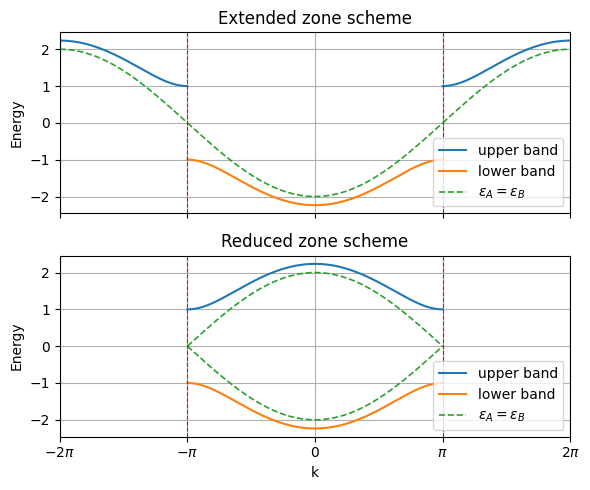
\includegraphics[width=0.5\linewidth]{dispersion11-2.png}
    \caption{Dispersion relations in the reduced and extended zone schemes. $t=1$, $\epsilon_A-\epsilon_B=2$ for orange and blue line and $t=1$, $\epsilon_A-\epsilon_B=0$ for green dashed line.} 
    \label{fig:dispersion-11-2}
\end{figure}

(d) In the atomic limit ($t\rightarrow 0$), the system reduces to two independent energy levels without coupling.
\begin{equation}
    E_+=\epsilon_A,\quad E_-=\epsilon_B.
\end{equation}


(e) For the lower band, the Taylor expansion is:
\begin{equation}
    E_-(k)=E_-(0) + \frac{t^2}{\sqrt{(\epsilon_A-\epsilon_B)^2/4 + 4t^2}}\frac{k^2}{2}.
\end{equation}
Hence, the effective mass is 
\begin{equation}
    \frac{\hbar^2k^2}{2m_\text{eff}}=\frac{t^2}{\sqrt{(\epsilon_A-\epsilon_B)^2/4 + 4t^2}}\frac{(ka)^2}{2}\Rightarrow m_\text{eff}=\frac{\hbar^2\sqrt{(\epsilon_A-\epsilon_B)^2/4 + 4t^2}}{a^2t^2}
\end{equation}

(f) If the atoms are monovalent, since there are two modes for one momentum eigenstate, spin $\pm1/2$, they only fill the lower band. Due to the energy gap between the lower and upper bands, the system is insensitive to external perturbations, thus behaving as an insulator.

(g) The crystal structure of LiF is shown in Figure.~\ref{fig:lif}. If a layer in $xy$ is considered as an atom with multiple modes, it also has lattice translation symmetry as the same as the 1D diatomic chain. Hence, there are gaps between the filled lower band and the unfilled upper band. Due to the gap, the LiF crystal is also insensitive to external perturbations, and it can be a good insulator.

\begin{figure}[b]
    \centering
    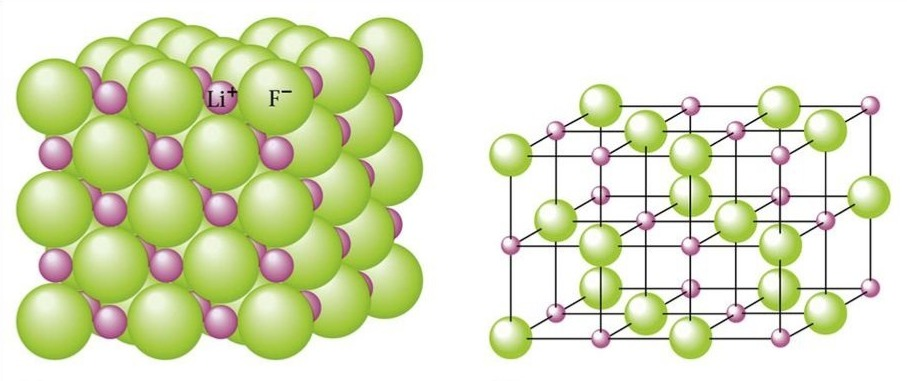
\includegraphics[width=0.35\linewidth]{LiFStructure.jpg}
    \caption{LiF crystal}
    \label{fig:lif}
\end{figure}


\section{11.5 Electronic Impurity State}

(a)

\begin{equation}
    \sum_{m}H_{n, m} \phi_m = A\left[\epsilon_0e^{-qa|n|}-t\left(e^{-qa|n+1|}+e^{-qa|n-1|}\right)+\delta_{n, 0}\Delta\right]
\end{equation}

To be an eigenstate,
\begin{gather}
    \sum_m H_{n, m}\phi_m = E\phi_n \\
    -t\left(e^{-qa|n+1|}+e^{-qa|n-1|}\right) + \delta_{n0}\Delta = (E-\epsilon)e^{-qa|n|}
\end{gather}

\begin{align}
    n=0:&& -2te^{-qa}+\Delta&=E-\epsilon \\
    n>0:&& -t\left(e^{qa}+e^{-qa}\right)e^{-qan}&=(E-\epsilon)e^{-qan} \\
    n<0:&& -t\left(e^{-qa}+e^{qa}\right)e^{qan}&=(E-\epsilon)e^{qan}
\end{align}

Hence there are two conditions:
\begin{equation}
    \begin{cases}
        -2te^{-qa} + \Delta = E-\epsilon \\
        -t(e^{qa}+e^{-qa})=E-\epsilon
    \end{cases}
\end{equation}

Therefore,
\begin{equation}
    \sinh qa = -\frac{\Delta}{2t},\quad E = \epsilon_0-2t\cosh qa = \epsilon_0-2t\sqrt{1+\frac{\Delta^2}{4t^2}}
\end{equation}

If $\Delta$ is negative, there exists a positive $q$ such that it satisfies the eigenvalue equation and the eigenstate is localized at $n=0$ because the amplitude is decaying exponentially as $n\rightarrow \infty$ if $q$ is positive.

The normalized eigenstate is
\begin{equation}
    \frac{\sqrt{-\Delta}}{(4t^2+\Delta^2)^{1/4}}\sum_{n=-\infty}^{\infty}e^{\operatorname{arsinh}(\Delta/2t)|n|}\ket{n}
\end{equation}

(b) Hamiltonian:
\begin{equation}
    H = -\frac{\hbar^2}{2m^*}\partial_x^2 +(a\Delta)\delta(x)
\end{equation}

Eigenvalue equation:
\begin{equation}
    -\frac{\hbar^2}{2m^*}\psi''(x) +(a\Delta)\delta(x)\psi(x) = E\psi(x)
\end{equation}

For the two pieces, $x<0$, $x>0$,
\begin{equation}
    \psi''(x)=\frac{2m^* (-E)}{\hbar^2}\psi(x)
\end{equation}

For the localized bounded state, $E<0$. Hence $-E>0$. Therefore the solutions are exponential functions:
\begin{equation}
    e^{qx},\quad e^{-qx}
\end{equation}
Where $q = \frac{\sqrt{2m(-E)}}{\hbar}$, $E=-\frac{\hbar^2q^2}{2m^*}$

A physically acceptable (normalizable) solution cannot diverge as $x \rightarrow \pm\infty$. Hence we can write the solution as
\begin{equation}
    \psi(x)=\begin{cases}
        Ae^{qx} & \text{if $x < 0$} \\
        Be^{-qx} & \text{if $x > 0$}
    \end{cases}
\end{equation}
for positive $q$.

Continuity condition:
\begin{equation}
    \psi(0+)=\psi(0-)
\end{equation}
Therefore, $A=B$

Condition for first derivative:
\begin{align}
    \psi'(+\varepsilon)-\psi'(-\varepsilon) 
    &= \int_{-\varepsilon}^{\varepsilon} \psi''(x) dx \\
    &= \int_{-\varepsilon}^{\varepsilon} dx \left[\frac{2m^*(a\Delta)}{\hbar^2}\delta(x)\psi(x)-\frac{2m^*E}{\hbar^2}\psi(x)\right] \\
    &=\frac{2m^*(a\Delta)}{\hbar^2}\psi(0)-\frac{2m^* E}{\hbar^2}\int_{-\varepsilon}^{\varepsilon}\psi(x)\, dx
\end{align}

as $\varepsilon\rightarrow 0+$, $\int_{-\varepsilon}^{\varepsilon}\psi(x)\, dx\rightarrow 0$. Hence the condition is
\begin{equation}
    \psi'(+0)-\psi'(-0)=\frac{2m^*(a\Delta)}{\hbar^2}\psi(0)
\end{equation}

Therefore,
\begin{equation}
-qA-qA = \frac{2m^*(a\Delta)}{\hbar^2}A\Rightarrow q=-\frac{m^*a\Delta}{\hbar^2}
\end{equation}
Since $q$ must be positive, we obtain the same constraint, $\Delta <0$.

Hence the normalized eigenfunction and the eigenenergy are:
\begin{equation}
    E=-\frac{m^*a^2\Delta^2}{2\hbar^2}, \quad\psi(x)=\sqrt{\frac{m^*a|\Delta|}{\hbar^2}}e^{\frac{m^* a\Delta}{\hbar^2}|x|}
\end{equation}

by replacing $m^*=\frac{\hbar^2}{2t a^2}$ and $x=na$,
\begin{equation}
    E=-\frac{\Delta^2}{4t},\quad\psi(na)=\sqrt{\frac{|\Delta|}{2ta}}e^{\frac{\Delta}{2t}|n|}
\end{equation}


if $\Delta /t$ is small enough
\begin{equation}
    \epsilon_0-2t\sqrt{1+\frac{\Delta^2}{4t^2}}=\epsilon_0-2t -\frac{\Delta^2}{4t}+O(\Delta^4)\approx(\text{constant})-\frac{\Delta^2}{4t}
\end{equation}
and
\begin{equation}
    \quad\psi(na)\propto e^{\frac{\Delta}{2t}|n|}\approx e^{\operatorname{arsinh}(\Delta/2t)|n|}
\end{equation}

The results are similar to the result of (a).



\section{11.8 Peierls Distortion}

\begin{equation*}
    \cdots =A-\underbrace{\overset{a}{A}=\overset{b}{A}}_{j-1}-\underbrace{\overset{a}{A}=\overset{b}{A}}_{j}-\underbrace{\overset{a}{A}=\overset{b}{A}}_{j+1}-A=\cdots
\end{equation*}

The Hamiltonian without spin will be:
\begin{align}
    H
    &=\left(-t_\text{short}\sum_j b_j^\dagger a_j -t_\text{long}\sum_j a_{j+1}^\dagger b_j \right)+\hc +\epsilon\sum_{j}(a_j^\dagger a_j+b_j^\dagger b_j)\\
    &=-t\sum_{j}((1+\varepsilon)b_{j}^\dagger a_j + (1-\varepsilon)a_{j+1}^\dagger b_j) + \hc + \epsilon\sum_j \left(a_j^\dagger a_j + b_j^\dagger b_j\right)
\end{align}

Perform the Fourier transformation:
\begin{equation}
    a_j=\frac{1}{\sqrt{N}}\sum_{k}e^{ikj}a_k,\quad 
    b_j=\frac{1}{\sqrt{N}}\sum_{k}e^{ikj}b_k
\end{equation}
Where $k=2\pi m/N, m\in\mathbb Z_N$

Then the Hamiltonian becomes
\begin{align}
    H
    &=-t\sum_{k}\left[(1+\varepsilon)b_k^\dagger a_k \right]+\hc -t\sum_{k}\left[(1-\varepsilon)a_k^\dagger b_k\right]+\hc +\epsilon\sum_k\left[a_k^\dagger a_k + b_k^\dagger b_k\right] \\
    &= \sum_k\begin{pmatrix}
        a_k^\dagger & b_k^\dagger
    \end{pmatrix}
    \begin{pmatrix}
        \epsilon & -t[(1+\varepsilon) + (1-\varepsilon)e^{-ik}] \\
        -t[(1+\varepsilon) + (1-\varepsilon)e^{ik}] & \epsilon
    \end{pmatrix}
    \begin{pmatrix}
        a_k\\b_k
    \end{pmatrix}
\end{align}

(a) Each mode can be diagonalized by
\begin{align}
    H(k)
    &=\begin{pmatrix}
        \epsilon & -t[(1+\varepsilon) + (1-\varepsilon)e^{-ik}] \\
        -t[(1+\varepsilon) + (1-\varepsilon)e^{ik}] & \epsilon
    \end{pmatrix}\\
    &=U\begin{pmatrix}
        E_+ & 0\\
        0 & E_-
    \end{pmatrix}U^\dagger
\end{align}
Where 
\begin{gather}
        E_\pm = \epsilon \pm 2t\sqrt{\cos^2\frac{k}{2}+ \varepsilon^2\sin^2\frac{k}{2}}, \quad U=\frac{1}{\sqrt 2}\begin{pmatrix}
        1 & -e^{-i\phi} \\
        e^{i\phi} & 1
    \end{pmatrix} \\
    \phi = \arg\left[-t(1+\varepsilon) - t(1-\varepsilon)e^{ik}\right]
\end{gather}
(b) The linear approximation of the band is
\begin{equation}
    E_\pm(k)=\epsilon \pm 2t\left|\cos \frac{k}{2}\right| + O(\varepsilon^2)
\end{equation}
It reduced to the result of the normal tight-binding chain.

For the second-order expansion,
\begin{equation}
    E_\pm(k)=\epsilon \pm 2t\left[\left|\cos \frac{k}{2}\right| + \frac{\sin^2(k/2)}{2\left|\cos (k/2)\right|}\varepsilon^2\right] + O(\varepsilon^4)
\end{equation}

(c) Since the electrons are spin-1/2, there are two modes, $\sigma=\pm1/2$, for each eigenmode of momentum. Therefore, to be half-filled, it must be monovalent. 

(d) At half-filling, the lower band is fully occupied in the ground state. The ground state energy is
\begin{align}
    E_\text{GS}
    &=2\cdot (N/2)\epsilon - 2t\sum_{k,\sigma}\sqrt{\cos^2\frac{k}{2}+ \varepsilon^2\sin^2\frac{k}{2}} \\
    &=N\epsilon - 2t\sum_\sigma\frac{N/2}{2\pi}\int_{-\pi}^{\pi}dk\sqrt{\cos^2\frac{k}{2}+ \varepsilon^2\sin^2\frac{k}{2}} \\
    &=N\left[\epsilon-\frac{4t}{\pi}E\left(\sqrt{1-\varepsilon^2}\right) \right]
\end{align}
where $N$ is number of atoms and $E(m)=\int_0^{\pi/2} \sqrt{1-m^2\sin^2\theta} \, d\theta$ is the complete elliptic integral of the second kind. For $N$ atoms, there are $N/2$ unit cells and there are two-fold degeneracy for spin-1/2 states. Hence they cancel each other at the second and third equality. The thermodynamic limit was employed to replace the summation with an integral.

(e) Let's expand the elliptic integral near $1$. 
\begin{equation}
    E\left(\sqrt{1-\varepsilon^2}\right)=1-\frac{\varepsilon^2}{2}\left[\log \varepsilon+\frac{1}{2}-2\log 2\right] + \cdots
\end{equation}
Hence the approximation of the ground state energy is
\begin{equation}
     \frac{E_\text{GS}}{N}=\epsilon-\frac{4t}{\pi}+\frac{2t\varepsilon^2}{\pi}\left[\log \varepsilon+\frac{1}{2}-2\log 2\right] + \cdots
\end{equation}


(f) The potential energy is 
\begin{equation}
    \Delta E_\text{spring}(\delta x)=\sum_{j} \frac{1}{2} \kappa(2\delta x)^2=2N\kappa(\delta x)^2\propto (\delta x)^2
\end{equation}

(g) Assume $\epsilon$ is linearly proportional to $\delta x$.
Then the total energy change due to the distortion is
\begin{align}
    \frac{\Delta E_\text{GS}(\delta x)}{N} + \frac{\Delta E_\text{spring}(\delta x)}{N} 
    &= \frac{2\alpha ^2t(\delta x)^2}{\pi}\left[\log (\alpha\delta x)+\frac{1}{2}-2\log 2\right] + 2\kappa (\delta x)^2 \\
    &=A\delta x^2\log\delta x + B\delta x^2
\end{align}
Where $A=2\alpha^2 t/\pi$, $B=(2\alpha^2 t/\pi)[1/2 +\log (\alpha/4)] + 2\kappa$.

And this function has a local minimum at $\delta x=\exp\left(-\frac{A+2B}{2A}\right) > 0$. Therefore, the atomic chain spontaneously distort.




\section{11.9 Tight Binding in 2d}



Consider a 2D lattice with width $N_1$ and height $N_2$. The Hamiltonian of this system is
\begin{equation}
    H=-t_1\sum_{\sigma, x, y}c_\sigma^\dagger(x + 1, y)c_\sigma(x, y)+\hc-t_2\sum_{\sigma, x, y}c_\sigma^\dagger(x, y+1)c_\sigma(x, y)+\hc 
\end{equation}
sum over $x\in \mathbb Z_{N_1}$, $y\in \mathbb Z_{N_2}$, and $\sigma=\uparrow, \downarrow$.

Assuming periodic boundary conditions, $c_\sigma(N_1, y)=c_\sigma(0, y)$, $c_\sigma(x, N_2)=c_\sigma(x, 0)$, the system exhibits lattice translational symmetry. Thus, we apply a two-dimensional Fourier transform to diagonalize the Hamiltonian:
\begin{equation}
    c_\sigma(x, y) = \frac{1}{\sqrt{V}}\sum_{k_x, k_y}e^{i(k_xx + k_y y)}c_\sigma(k_x, k_y)
\end{equation}
Where $V=N_1N_2$.

Then the hamiltonian becomes:

\begin{equation}
    H=\sum_{k_x, k_y,\sigma}\epsilon(k_x, k_y)c_\sigma^\dagger (k_x, k_y) c_\sigma (k_x, k_y)
\end{equation}
Where $\epsilon(k_x, k_y)=-2t_1\cos k_x -2t_2 \cos k_y$

At to bottom of the band,
\begin{equation}
    \epsilon(k_x, k_y)\approx-2t_1-2t_2 + t_1k_x^2 + t_2k_y^2
\end{equation}

The dispersion relation is shown at Figure.~\ref{fig:2d-dis}.

\begin{figure}[b!]
    \centering
    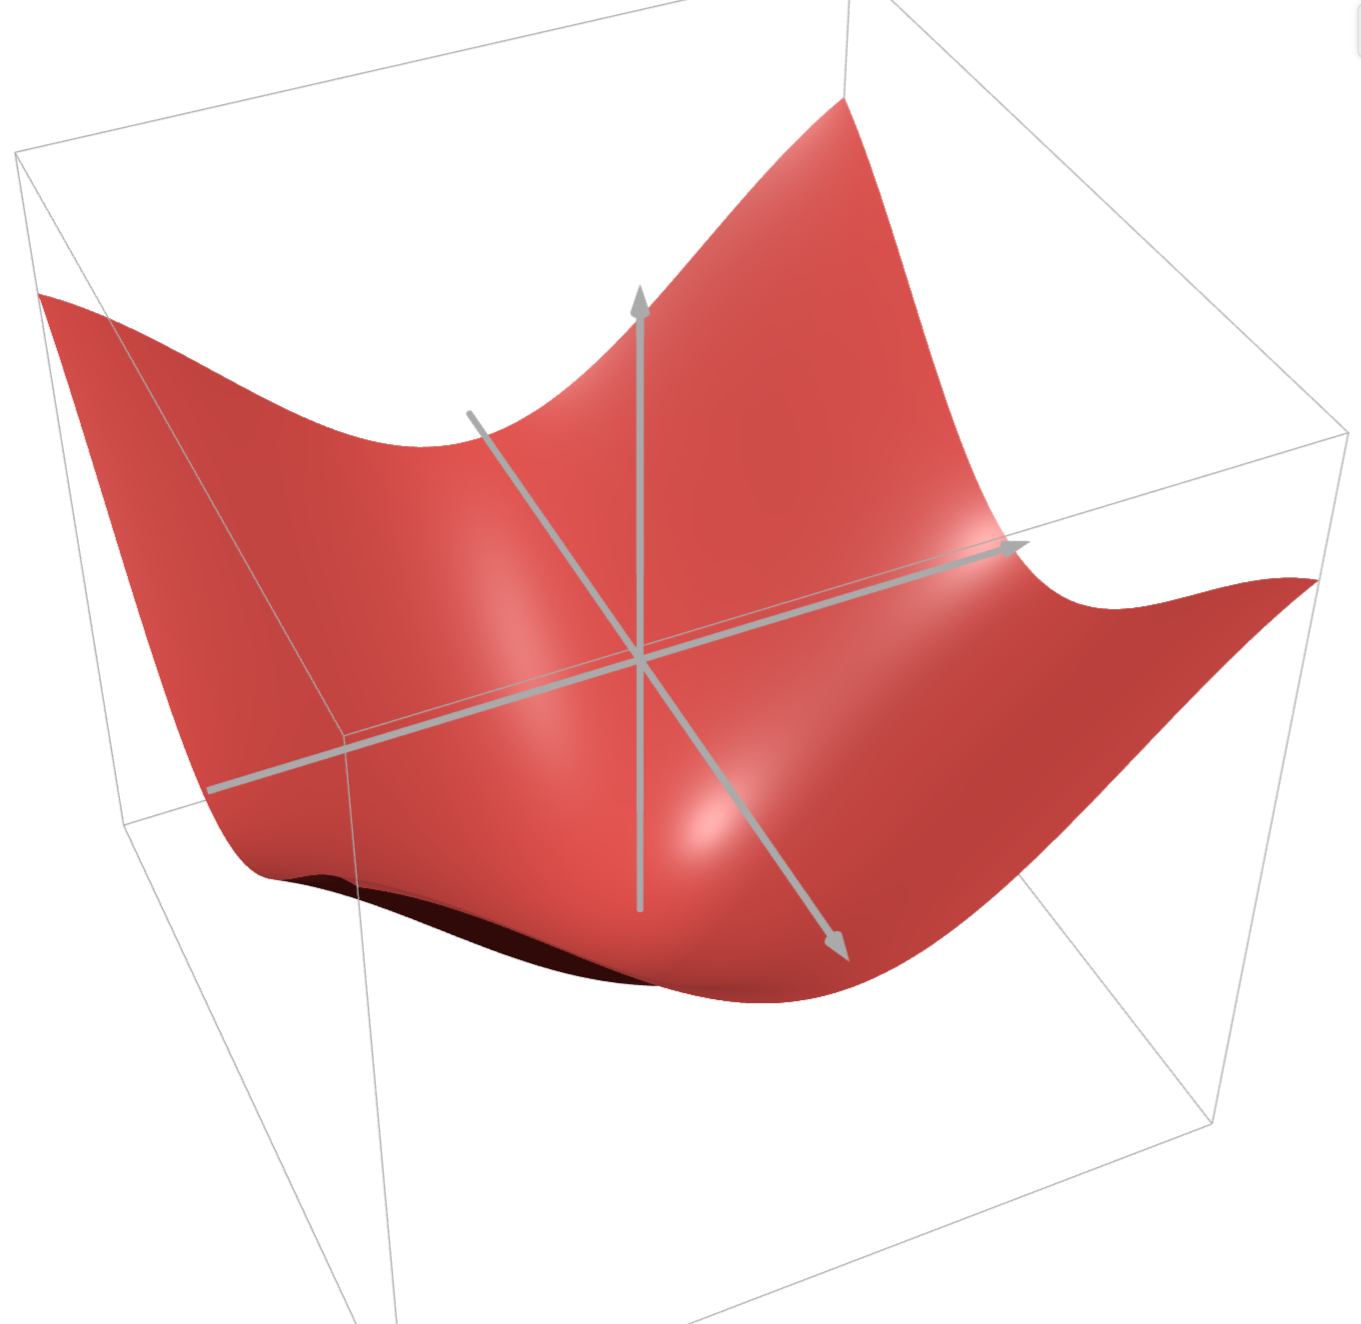
\includegraphics[width=0.5\linewidth]{2D tight-binding dispersion.png}
    \caption{Dispersion relation for 2D tight-binding model}
    \label{fig:2d-dis}
\end{figure}




\section{12.3 Crystal Structure}

.

(a) Both Zn and S atoms form a face-centered cubic lattice structure.


(b) A basis is a $\mathrm{Zn}$ atom at $(0, 0, 0)$ and a $\mathrm{S}$ atom at $(1/4, 1/4, 3/4)$.


(c) For $\mathrm{Zn}$ at $(0, 0, 0)$, the nearest $\mathrm{Zn}$ atoms are those at $(\pm1/2, \pm1/2, 0)$, $(\pm1/2, 0, \pm1/2)$ and $(0, \pm1/2, \pm1/2)$, total 12 atoms. The distance from $(0, 0, 0)$ is $\sqrt{2}a/2\approx0.3825\ \mathrm{nm}$. The nearest $\mathrm{S}$ atoms are those at $(1/4, 1/4, -1/4)$, $(1/4, -1/4, 1/4)$, $(-1/4, 1/4,1/4)$, and $(-1/4, -1/4, -1/4)$. The distance from (0, 0, 0) is $\sqrt3 a/4\approx 0.2343\ \mathrm{nm}$. The nearest S-S distance is equal to the Zn-Zn distance. Therefore,

\begin{enumerate}
    \item $\mathrm{Zn}-\mathrm{Zn}$: $\sqrt{2}a/2\approx0.383\ \mathrm{nm}$
    \item $\mathrm{Zn}-\mathrm{S}$: $\sqrt3 a/4\approx 0.234\ \mathrm{nm}$
    \item $\mathrm{S}-\mathrm{S}$: $\sqrt{2}a/2\approx0.383\ \mathrm{nm}$
\end{enumerate}






\end{document}
